\section{Results}

% 1 page
%Renan: Results-Intro
%TODO Gabriel: Results-Calibration
%Estevão: Results-Mecanica
%Renan: Results-Control

% Intro

Simulations and experimental tests at Jirau's facility were performed to verify
the proposed concepts. The results are divided according to the EMMA system's
elements introduced in Sec.~\ref{solution}. 

\subsection{Robotic manipulator analysis}\label{sec::man_analysis}

As stated in Subsec.~\ref{manipulator}, simulations for the robotic
manipulator were implemented with OpenRave, and consist of the following steps:
blade's surface discretization; base position computation; kinematics
and dynamics.

A survey of off-the-shelf manipulators was conducted for
Jirau's turbine. Regarding the runner's blade dimension, among the analyzed
mid-sized robotic manipulators, the Yaskawa Motoman MH12 robot was chosen due to its satisfactory
workspace, and versatility. Blade discretization is performed in a Jirau
runner's blade CAD model, Fig.~\ref{fig:discretization} shows the blade's
samples, and Fig.~\ref{fig:coating} shows the manipulator workspace, where
black dots are coated points and blue dots are coated points with the angle
tolerance. Thus it is possible to create a coating strategy and to select the
simplest base positions. The result is the minimum required positions for the
robotic manipulator's base.

\begin{figure}
	\centering
	\subfigure[Blade
	discretization]{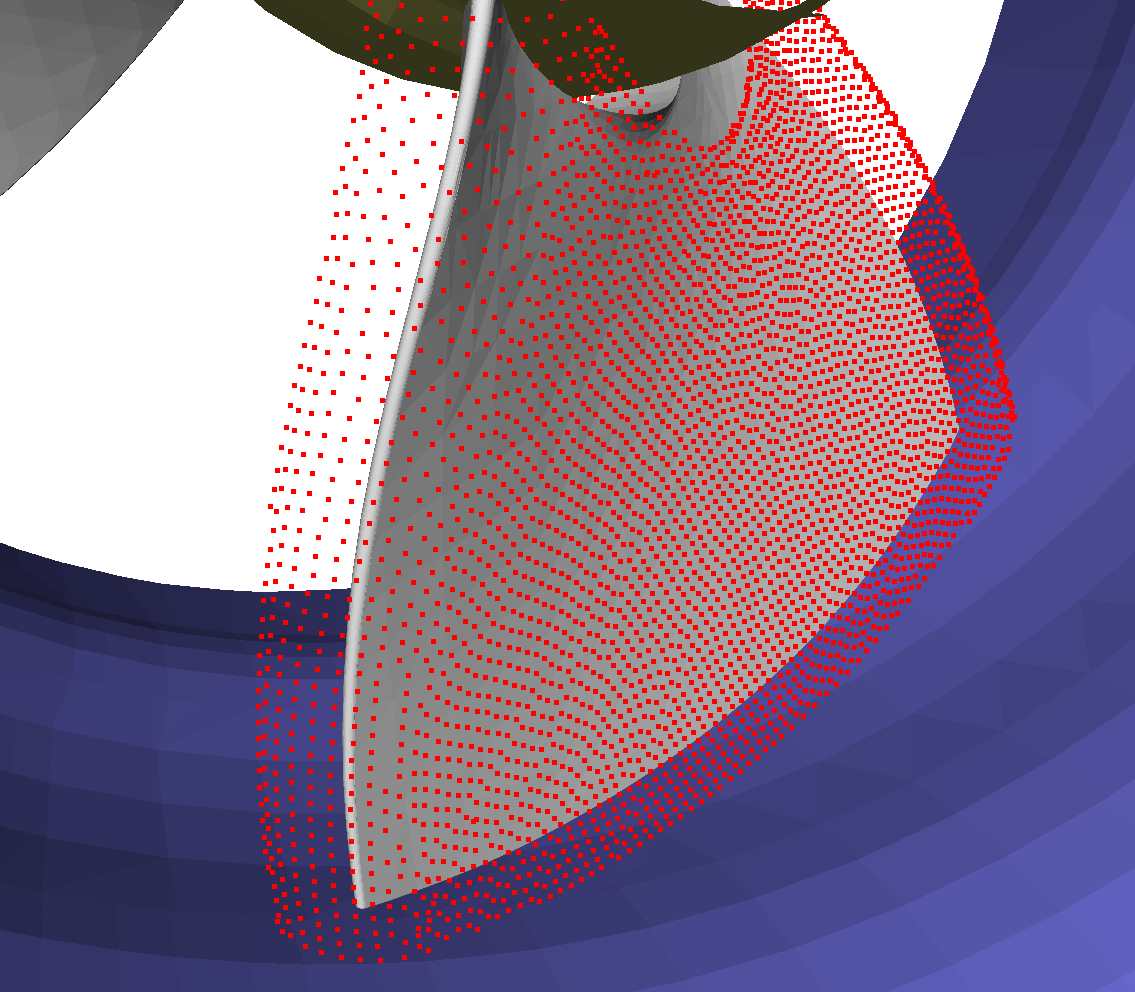
\includegraphics[width=0.46\columnwidth]{figs/results/blade_grid1.png}\label{fig:discretization}}
	\quad
	\subfigure[Manipulator
	workspace]{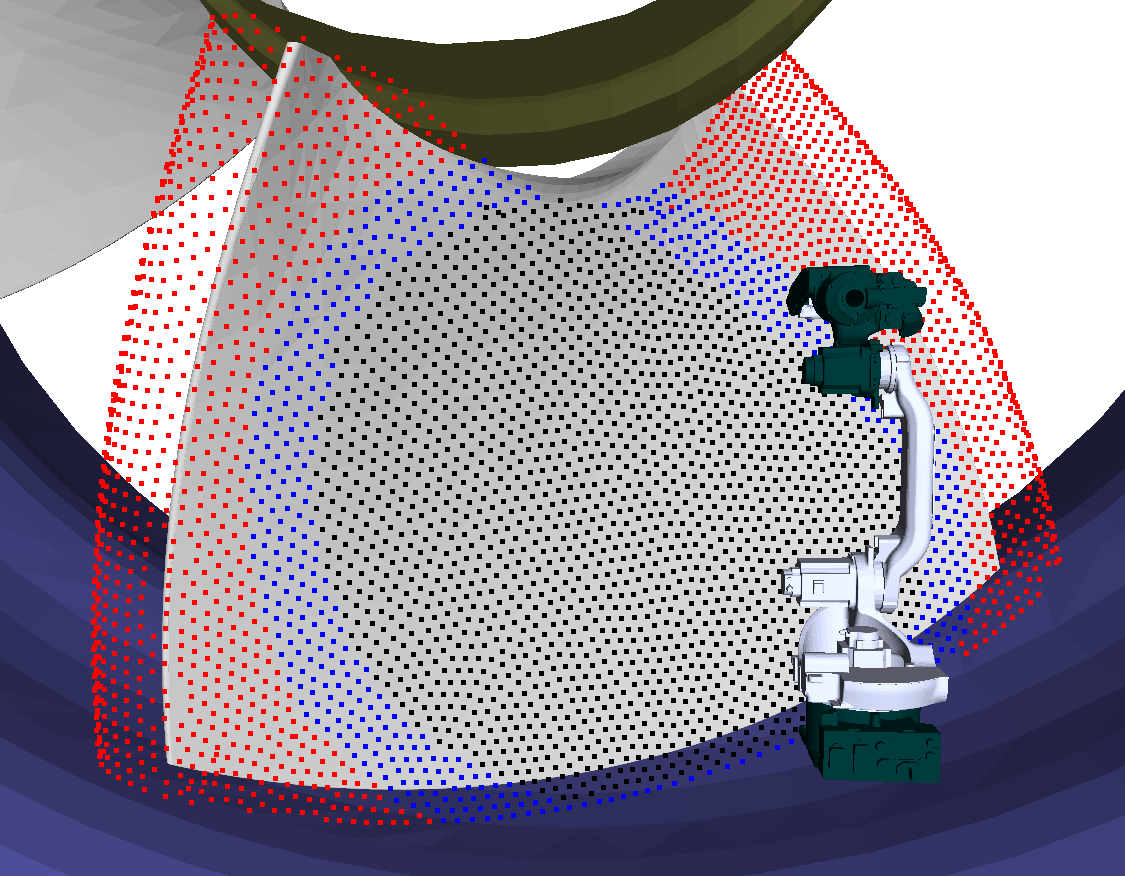
\includegraphics[width=0.47\columnwidth]{figs/results/mh12_coating2.png}\label{fig:coating}}
	\caption{Blade discretization and manipulator workspace for a fixed position.}
\end{figure}

Comparing estimated torques with the technical specifications, dynamic
simulations' results showed that the robotic manipulator should be placed at,
at least, 1400~mm distance from the blade's surface plane. Placing the robot
nearer would enhance the robotic manipulator's workspace, but it would increase
also the torques. 

\begin{comment}
The Fig.~\ref{fig:torques} is an example of the robotic
manipulator in a close range, 900~mm distance from the blade. It shows joints'
torques in a color gradient way, where red dots represents small magnitudes and
blue dots are large.

\begin{figure}
	\centering
	\includegraphics[width=.5\columnwidth]{figs/results/manipulability_colorgradient.png}
    \caption{Robotic manipulator joints' torques in color gradient.}
    \label{fig:torques}
\end{figure}
\end{comment}

Despite being able to coat approximately 50\% of the blade on a fixed
position, kinematic and dynamic analysis show that the MH12 robot cannot fully
cover it vertically or horizontally, demanding extra 2-DOF along the blade's
surface. The base position computations reveal that the blade's top
extremities require a specific base position, reachable
with a primary rail between the blades. Therefore, the MH12 robot will require
at least four positions along the blade and one position on a primary
rail, between blades. 

\subsection{Mechanical system analysis}

In the specific case of Jirau, the secondary rail is customized with a third
prismatic joint for height adjustment of the robotic manipulator. The primary
and secondary rails with extra DOF guarantee the full coating, as they allow the
robotic manipulator movement in the confined space by a 4-DOF base, PRPP joints.

The FEA of the base verifies the Von Mises stress and the displacements
along the structure's slender members. The stress analysis determines the
integrity of the base due to the maximum loads of the robotic manipulator. The
displacements determine if the structure provides a rigid base for the robotic
manipulator. According to the hard coating requirements, displacements of the
order of millimeters are not allowable in the elastic region of the
material. 

The FEA solver was the Nastran In-CAD$^{\mbox{\small\textregistered}}$ with
SolidWorks$^{\mbox{\small\textregistered}}$. Model's elements are 1-D 
\textit{bar line elements} with a global mesh's size of 25~mm. The material's
properties are: density 2700~$kg/m^3$; Young modulus 70~GPa; Poisson's ratio
0.34; and Yield strength 200~MPa. Boundary conditions are three translational
constraints for the anchors and a vertical constraint to the feet. The
rotational joint is modeled as a rigid connector between the rails, such as the
robot's base with respect to the second rail. The robotic manipulator's maximum
dynamic forces and moments are applied, as static loads, to the point that
represents the origin of the robot's base.

The maximum Von Mises stress was 4.16~MPa (Fig.~\ref{fig:von_mises}), which
gives a factor of safety of 34.6. It was found for a particular case where the robotic manipulator is in
the secondary rail, 800~mm from the rotational joint. The displacement of the
structure causes a maximum translation of 0.47~mm and a angular deflection of
$0.0149^{\circ}$ in respect to robotic manipulator base's coordinate system. 

The field tests conducted in the draft tube for the magnetic fixtures, at
different equipment's orientations and places, confirmed the manufacturer's
payload capacity. As the maximum tractive reaction force obtained in FEA
simulations was 956~kgf, it was chosen a magnetic fixture with 1200~kgf
payload capacity.

\begin{figure}
	\centering
	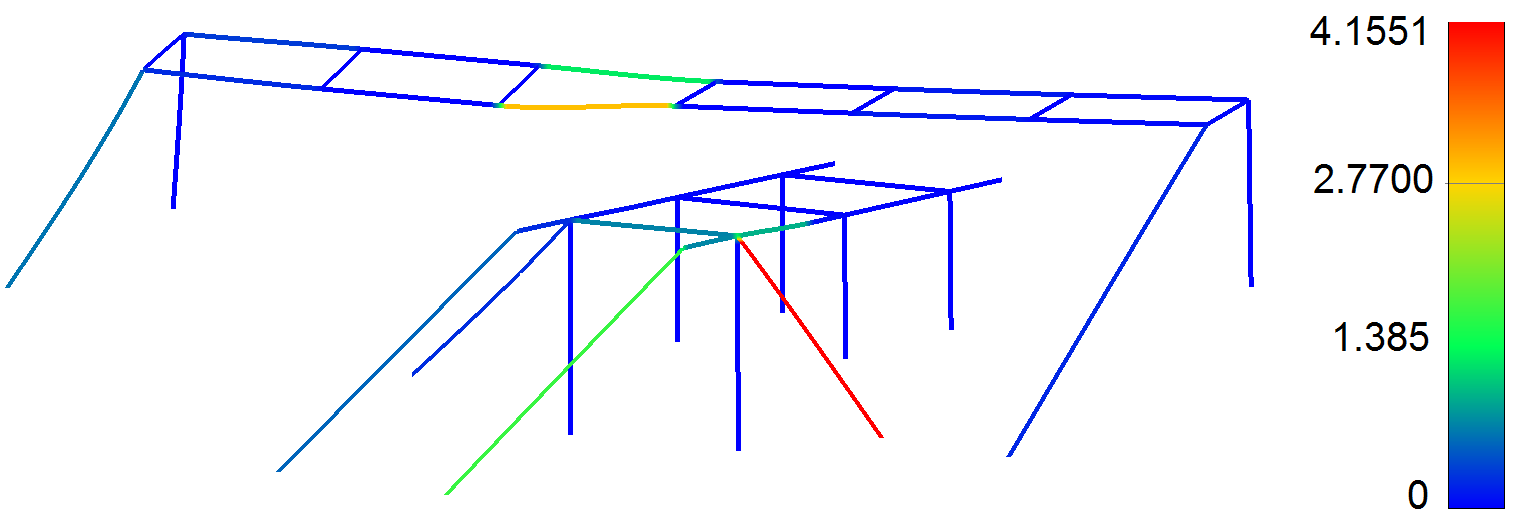
\includegraphics[width=.95\columnwidth]{figs/mecanica/von_mises.png}
    \caption{Von Mises's stress result.}
    \label{fig:von_mises}
\end{figure}

\subsection{Calibration analysis}

To test the calibration algorithm for the blades, the turbine
environment and the robotic manipulator were simulated with help of the toolbox
Blensor \cite{Gschwandtner11b} and based on the technical drawings from the
powerplant. The blade model, however, was acquired in a field test by a 3D laser
scanner for a better representantion of the actual hidraulic profile.

The laser sensor was modeled following manufacturer's technical
specifications, and different scenes were generated for several sensor
positions. The algorithm is able to localize the blade in respect to the
sensor's coordinate system, even in occlusion generated by the presence of the
robotic manipulator. In Fig.~\ref{fig:calibration}, it can be seen the
correspondeces between the reference model and the scene, or the turbine
environment, and also the correctly localized blade instance highlighted in red.

\begin{figure}
	\centering
	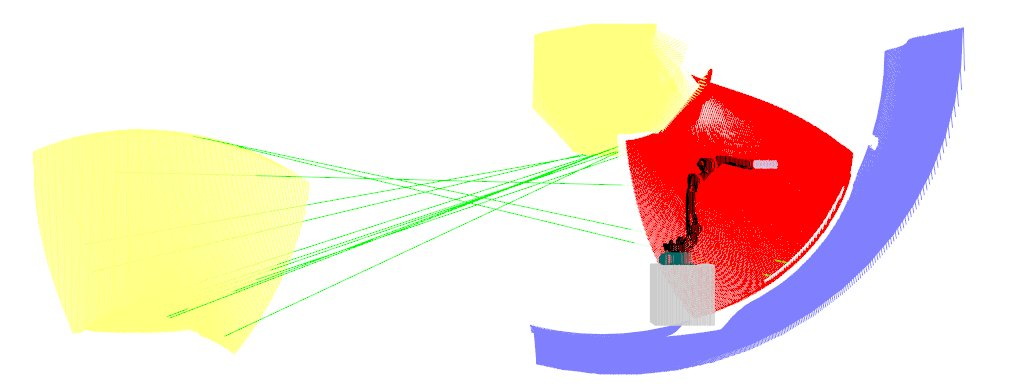
\includegraphics[width=.95\columnwidth]{figs/results/sim_mh12_sp}
    \caption{Blade reference model localized in the turbine environment with
    occlusions.}
    \label{fig:calibration}
\end{figure}

The Fig. \ref{fig:histogram} exemplifies the error or distance distribution
to the closest point from the scene to each point of the model. The mean
distance between each swipe of the laser scan is $9~mm$ and the
RMS error is $4~mm$, which is consistent as the half of the resolution of the
point clouds.

\begin{figure}
	\centering
	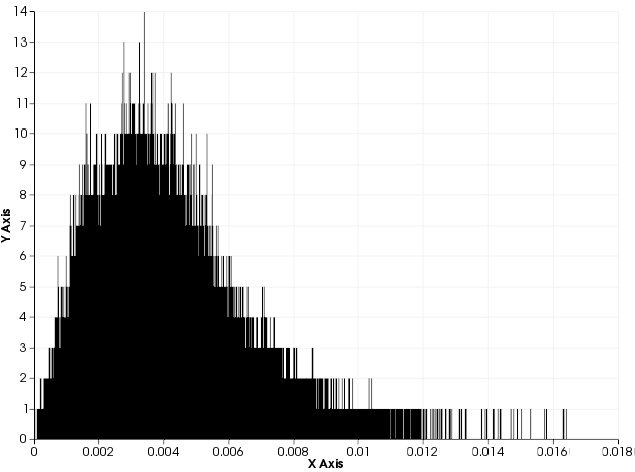
\includegraphics[width=.95\columnwidth]{figs/results/histogram}
    \caption{Histogram of the error (meters) between the model and reference
    scene point to point.}
    \label{fig:histogram}
\end{figure}

Similar procedure was followed to recreate a scene with four reference spheres
(supposedly attached to the robot). The 3D Hough Method was able to locate all
spheres' centers within a $5mm$ error (fig. \ref{fig:sphere_hough}).

\begin{figure}
	\centering
	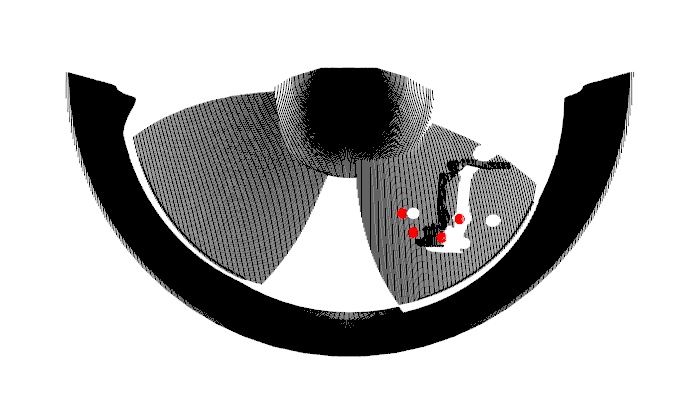
\includegraphics[width=.95\columnwidth]{figs/results/SphereHough}
    \caption{Points recognized as belonging to the four spheres (in red).}
    \label{fig:sphere_hough}
\end{figure}

